\section{Methods}   \label{sec:methods}

IMU measurements provide the arm's orientation at given spots along the arm. 
This section will discuss how to use this data  to estimate the full arm shape using two different arm parametrizations.
For both of the presented models, the arm is parameterized as a series of rigid segments. 

In part \ref{rigid body model}, one segment per IMU is used. 
In part \ref{pseudo-PCC rigid body model}, we use spherical linear interpolation to create ``virtual IMUs" to increase the number of segments without increasing the number of IMUs. 
% This method approximates piece-wise constant curvature model (PCC).
In the limit, this method approximates a Piecewise Constant Curvature model (PCC) \cite{webster2010_pcc}. Both models are constructed from IMU orientation data in the form of quaternions, which are singularity free, as opposed to Euler angles which suffer from the Gimbal Lock issue \cite{doi:10.1177/003754976500400610}.
Quaternions are also broadly used in computer science and as a default IMU output format.

The models specify the shape of the arm as a collection of joint coordinates.
However, because both models represent the arm as a series of rigid segments, it is straightforward to compute the coordinates of any point along the length of the arm using linear interpolation between two adjacent joints.
% The formulas are given only for the edges of the segments, but it is easy to compute any data point along the arm using linear interpolation between the two adjacent edges. 

\subsection{Rigid-body model} \label{rigid body model}
% Here will be presented a mathematical model for Fig. \ref{models}(a)
The arm is modeled by $N+1$ straight links of length $L^R_i \text{, } i \in \{0,...,N\}$, called segments (see Fig.~\ref{models}(a)). 
An IMU is fixed to each segment, ideally on the center.
The $i^{th}$ segment is oriented along the IMU frame defined by its quaternion $\mathbf{q_i}$, $i \in \{0,...,N\}$ where
$\mathbf{q_0}$ is the orientation of the arm's base.
We define $R_q(\mathbf{q})$ as the 3x3 rotation matrix extracted from a quaternion $\mathbf{q} = a + i b + j c + k d$ \cite{tf_lib_ROS},

\begin{equation}
    R_q(\mathbf{q}) = \begin{pmatrix} 1 - 2(c^2+d^2) & 2(b c-a d) & 2(b d + a c) \\ 
    2(b c + a d) & 1 - 2(b^2 + d^2) & 2(c d - a b) \\
    2(b d - a c) & 2(c d + a b) & 1 - 2(b^2 + c^2) \end{pmatrix}
\end{equation}

Let $\mathbf{\hat{x}^{R}_i}$ be an estimate of the position of the joint between segment $i$ and segment $(i-1)$ according to this model.
It is computed by summing the displacements of the first $i-1$ links, according to the following expression,


\begin{equation}
    \mathbf{\hat{x}^{R}_i} =  \sum_{j=0}^{i-1} R_q(\mathbf{q_j}) \begin{pmatrix} 0 \\0 \\ L^R_j \end{pmatrix}
       \label{formula_rigid_body_model_2}
\end{equation}
Note that the superscript $(\cdot)^R$ denotes a variable related to the rigid-body model.

\subsection{PCC-extended rigid-body model} \label{pseudo-PCC rigid body model}

To make the rigid-body model smoother and more accurate, we divide each segment into $n$ sub-segments.
Each sub-segment orientation is computed under the assumption that the segment's curvature is constant.
As $n$ increases, this model approximates a PCC model.

Let us define $L^E_i$ as the distance between $\mathbf{q_i}$ and $\mathbf{q_{i+1}}$,
%
and $\mathbf{q_{i,k}}$ as the orientation quaternion of the $k^{th}$ sub-segment of the $i^{th}$ segment (see Fig.~\ref{models}(b)), which is computed using spherical linear interpolation between $\mathbf{q_i}$ and $\mathbf{q_{i+1}}$.

\begin{equation}
    \mathbf{q_{i,k}}=slerp\left(\mathbf{q_i},\mathbf{q_{i+1}},\frac{2k+1}{2n}\right)
\end{equation}
The function $slerp$ represents spherical linear interpolation \cite{fast_slerp} and is defined as,
\begin{equation}
slerp(\mathbf{q_a},\mathbf{q_b},t) = (\mathbf{q_b} \mathbf{q_a}^{-1})^t \mathbf{q_a}
\end{equation}
where $t \in [0,1]$ is the interpolation variable such that $slerp(\mathbf{q_a},\mathbf{q_b},0) = \mathbf{q_a}$ and $slerp(\mathbf{q_a},\mathbf{q_b},1) = \mathbf{q_b}$. \\

Next, the position of the $k^\text{th}$ joint of the $i^\text{th}$ segment, denoted $\mathbf{\hat{x}_{i,k}^E}$, is computed by summing the displacement of all preceding joints according to the following expression,
\begin{equation}
    \mathbf{\hat{x}_{i,k}^{E}} = \mathbf{\hat{x}_{i,0}^{E}} + \sum_{m=0}^{k-1} R_q(\mathbf{q_{i,m}})\begin{pmatrix} 0 \\0 \\  L^E_i/n \end{pmatrix} 
\end{equation}
Note that the superscript $(\cdot)^E$ denotes a variable related to the PCC-extended rigid-body model.
%

We define the $0^{th}$ joint of the $0^{th}$ segment to be located at the origin,
%
\begin{equation}
     \mathbf{\hat{x}_{0,0}^{E}} = \begin{pmatrix} 0 \\0 \\  0 \end{pmatrix} 
\end{equation}
and since the $n^{th}$ joint of segment $i$ is the same as the $0^{th}$ joint of segment $i+1$ the following are equivalent, 
%
\begin{equation}
   \mathbf{ \hat{x}_{i+1,0}^{E}} = \mathbf{\hat{x}_{i,n}^{E}}
\end{equation}
%


\begin{figure}
    \centering
    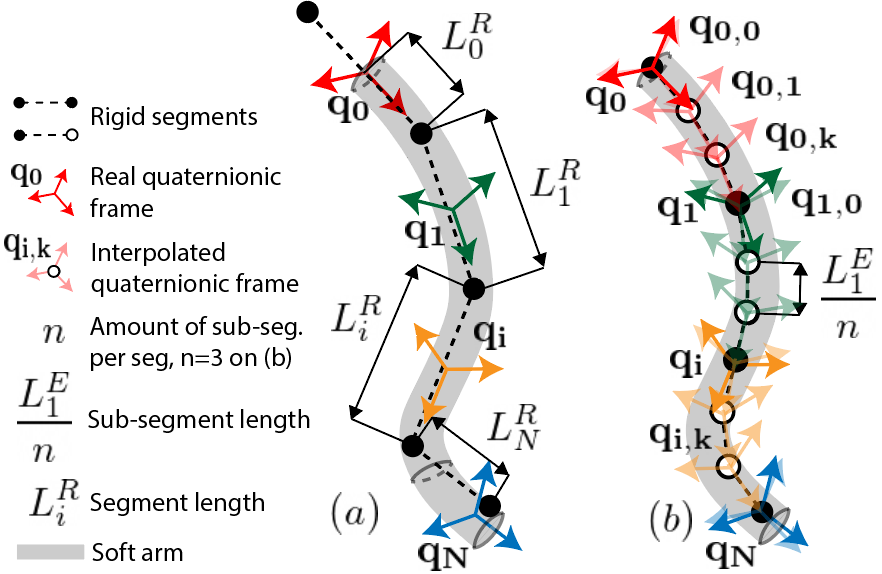
\includegraphics[width=\linewidth]{fig/models2.png}
    \caption{Different models to approximate the state of a soft continuum arm using IMUs: (a) rigid-body model, (b) and PCC-extended rigid-body model.}
    \label{models}
\end{figure}
